\documentclass[../besoin_user.tex]{subfiles}
\begin{document}
\section{En partie}
Le jeu doit être conçu pour offrir une interface intuitive, facilitant ainsi les actions du joueur.
Dans un premier temps, les deux joueurs sont invités à placer les bateaux sur le board.
Les bateaux qui sont disponibles varient du mode de jeu qui a été choisi.
Un message d'erreur est affiché lorsque le bateau est placé sur une mauvaise case et auquel cas le joueur est invité à 
essayer une autre position. Le même procédé sera utilisé pour les tirs.

Une fois tout les bateaux placés sur le board, le timer commence et la game débute.
Chacun des joueurs doit alors tirer sur une case du board de l'adversaire, et le jeu continue jusqu'à ce que l'un des joueurs ait coulé tous les bateaux de l'autre joueur.
Si un joueur touche un bateau, il a le droit de tirer une autre fois, sinon c'est au tour de l'autre joueur.
Pour rendre l'expérience en jeu plus agréable et plus interactive, le temps de jeu ne doit pas être trop long.

\begin{figure}[h]
    \centering
    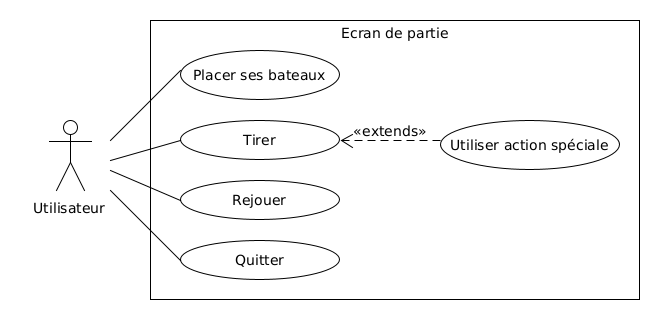
\includegraphics[scale=0.6]{img_fonctionnel/use_case_user_ecran_partie.png}
    \label{fig:user_partie}
    \caption{En partie}
\end{figure}

\subsection{Mode classique}
Le mode classique est le mode jeu original de la bataille navale. Chaque joueur doit placer 5 bateaux, qui sont les suivants:
\begin{itemize}
    \item 1 porte-avion (5 cases)
    \item 1 croiseur (4 cases)
    \item 2 sous-marin (3 cases)
    \item 1 torpilleur (2 cases)
\end{itemize}
Vous aurez remarqué que le contre-torpilleur n'est pas présent dans ce mode de jeu, mais que nous avons deux sous-marins. Cela s'explique car il n'est pas
dissociable du sous-marin dans nos modes d'affichages, nous avons alors fait le choix de le fusionner avec le sous-marin.

\subsection{Mode commandant}
Le mode commandant est un mode de jeu plus complexe, qui offre une expérience de jeu plus intense. Chaque joueur peut choisir entre les trois factions disponibles,
ce qui lui donnera des compétences spéciales, et une flotte de bateaux personnalisée. Cependant, toutes les factions commencent la partie avec une mine.

Tous les tours, les joueurs gagnent un point d'énergie. Avec cette énergie, le joueur peut utiliser une compétence spéciale.
Si un joueur touche une mine, il perd 3 points d'énergies. Si le joueur a une énergie négative, le joueur en question ne peut pas tirer pour ce tour.

Les capacités qui sont diponibles pour toutes les classes sont donc les suivantes:
\begin{itemize}
    \item[-] \textbf{Tir normal 1x1} - \textit{0 point d'énergie} : Le tir normal est le même que dans le mode classique. Il ne coûte pas d'énergie, mais il n'est pas disponible si l'énergie est négative.
    \item[-] \textbf{Sonar 3x3} - \textit{4 points d'énergie} : Le joueur peut utiliser un sonar pour savoir si une case est de l'eau ou non.
    \item[-] \textbf{Bombardement en ligne 4x1} - \textit{4 points d'énergie} : Le Bombardement en ligne est similiare au tir normal, mais il touche 4 cases en ligne.
    \item[-] \textbf{Bombardement de périmètre 4x4} - \textit{9 points d'énergie} : Le Bombardement de périmètre est similiare au tir normal, mais il touche les contours extérieurs d'un carré de 4x4.
\end{itemize}

\subsubsection{Faction Mine}
Cette faction est celle des spécialistes de la mine. Ils possèdent la flotte suivante:
\begin{itemize}
    \item 2 bateaux de 2x1
    \item 2 bateau de 3 cases au choix
    \item 1 bateau de 4 cases au choix
\end{itemize}
La compétence spéciale de cette faction est la suivante:
\begin{itemize}
    \item[-] \textbf{Pose de mine} - \textit{2 points d'énergie} : Le joueur peut poser une mine sur une case de son choix. Si un bateau adverse touche cette case, il perd 3 points d'énergie.
\end{itemize}
Cependant, cette faction \textbf{ne peut pas recevoir de bombardement de périmètre}.

\subsubsection{Faction Sonar}
Cette faction est celle des spécialistes du sonar. Ils possèdent la flotte suivante:
\begin{itemize}
    \item 3 bateau de 2x1
    \item 4 bateau de 3 cases au choix
\end{itemize}

Les compétences spéciales de cette faction est la suivante:
\begin{itemize}
    \item[-] \textbf{Sonar 3x3} - \textit{3 points d'énergie}
    \item[-] \textbf{Sonar 10x1} - \textit{4 points d'énergie} 
\end{itemize}

\subsubsection{Faction Bombardement}
Cette faction est celle des spécialistes du bombardement. Ils possèdent la flotte suivante:
\begin{itemize}
    \item 1 bateau de 2x1
    \item 1 bateau de 3 cases au choix
    \item 2 bateaux de 4 cases au choix
    \item 1 bateaux de 5 cases au choix
\end{itemize}

Les compétences spéciales de cette faction est la suivante:
\begin{itemize}
    \item[-] \textbf{Bombardement 2x2} - \textit{4 points d'énergie}
    \item[-] \textbf{Bombardement 4x4} - \textit{7 points d'énergie}
\end{itemize}
\end{document}